% Options for packages loaded elsewhere
\PassOptionsToPackage{unicode}{hyperref}
\PassOptionsToPackage{hyphens}{url}
\documentclass[
]{article}
\usepackage{xcolor}
\usepackage[margin=1in]{geometry}
\usepackage{amsmath,amssymb}
\setcounter{secnumdepth}{5}
\usepackage{iftex}
\ifPDFTeX
  \usepackage[T1]{fontenc}
  \usepackage[utf8]{inputenc}
  \usepackage{textcomp} % provide euro and other symbols
\else % if luatex or xetex
  \usepackage{unicode-math} % this also loads fontspec
  \defaultfontfeatures{Scale=MatchLowercase}
  \defaultfontfeatures[\rmfamily]{Ligatures=TeX,Scale=1}
\fi
\usepackage[tt=false]{libertine}
\ifPDFTeX\else
  \setmonofont[StylisticSet=3]{inconsolata}
  \setmathfont[Scale=MatchUppercase]{LibertinusMath-Regular.otf}
\fi
% Scalable fallback for legacy math alphabets used by article's title footnotes.
\DeclareFontShape{OML}{cmm}{m}{it}{<-> cmmi10}{}
\ifPDFTeX\else
  % xetex/luatex font selection
\fi
% Use upquote if available, for straight quotes in verbatim environments
\IfFileExists{upquote.sty}{\usepackage{upquote}}{}
\IfFileExists{microtype.sty}{% use microtype if available
  \usepackage[]{microtype}
  \UseMicrotypeSet[protrusion]{basicmath} % disable protrusion for tt fonts
}{}
\makeatletter
\@ifundefined{KOMAClassName}{% if non-KOMA class
  \IfFileExists{parskip.sty}{%
    \usepackage{parskip}
  }{% else
    \setlength{\parindent}{0pt}
    \setlength{\parskip}{6pt plus 2pt minus 1pt}}
}{% if KOMA class
  \KOMAoptions{parskip=half}}
\makeatother
\usepackage{longtable,booktabs,array}
\usepackage{calc} % for calculating minipage widths
% Correct order of tables after \paragraph or \subparagraph
\usepackage{etoolbox}
\makeatletter
\patchcmd\longtable{\par}{\if@noskipsec\mbox{}\fi\par}{}{}
\makeatother
% Allow footnotes in longtable head/foot
\IfFileExists{footnotehyper.sty}{\usepackage{footnotehyper}}{\usepackage{footnote}}
\makesavenoteenv{longtable}
\usepackage{graphicx}
\usepackage{algorithm}
\usepackage{algpseudocode}
\makeatletter
\newsavebox\pandoc@box
\newcommand*\pandocbounded[1]{% scales image to fit in text height/width
  \sbox\pandoc@box{#1}%
  \Gscale@div\@tempa{\textheight}{\dimexpr\ht\pandoc@box+\dp\pandoc@box\relax}%
  \Gscale@div\@tempb{\linewidth}{\wd\pandoc@box}%
  \ifdim\@tempb\p@<\@tempa\p@\let\@tempa\@tempb\fi% select the smaller of both
  \ifdim\@tempa\p@<\p@\scalebox{\@tempa}{\usebox\pandoc@box}%
  \else\usebox{\pandoc@box}%
  \fi%
}
% Set default figure placement to htbp
\def\fps@figure{htbp}
\makeatother
\setlength{\emergencystretch}{3em} % prevent overfull lines
\providecommand{\tightlist}{%
  \setlength{\itemsep}{0pt}\setlength{\parskip}{0pt}}
\usepackage[]{natbib}
\bibliographystyle{plainnat}
\usepackage{bookmark}
\IfFileExists{xurl.sty}{\usepackage{xurl}}{} % add URL line breaks if available
\urlstyle{same}
\hypersetup{
  pdftitle={Supplementary Material for Teaching in the Student's Terms},
  pdfauthor={Anonymous Author(s)},
  hidelinks,
  pdfcreator={LaTeX via pandoc}}

\title{Supplementary Material for Teaching in the Student's Terms}
\author{Anonymous Author(s)}
\date{}

\emergencystretch=2em
\begin{document}
\maketitle

\section{Construction and Implementation}
\label{app:construction}

This appendix records the predicate features, bank construction and
checking choices, and training details used by the method.

\begin{table}[t]
\centering\small
\caption{Frozen banks used in the reported experiments. Each originates
from 36 generation consultations; checking requests are additional.
The two MultiRoom banks share the same initial consultations.}
\label{tab:banks}
\begin{tabular}{@{}llllr@{}}
\toprule
Task & Student & Check & Action filter & Rules\\
\midrule
DoorKey & Both & Blind & None & 16\\
MultiRoom & PPO & None & None & 32\\
 & Count-PPO & Blind & None & 7\\
KeyCorridor & Both & Self-check & Before freezing & 28\\
Crafter & Both & Self-check & Runtime & 24\\
\bottomrule
\end{tabular}
\end{table}

\subsection{Predicate Features and Progress}
\label{app:predicate_features}

The final vocabularies are frozen before evaluated training. MiniGrid observation predicates describe the front
cell, carried object, visibility of task-relevant object types, coarse
direction and offsets to their closest visible instances, and visible
door states. The carried object is encoded at the agent's cell in the
symbolic observation. An unseen object's direction and offsets are
$\mathsf{unknown}$.
Crafter predicates describe the facing cell and direction, daylight,
nearby table and furnace, distance and first move towards the closest
visible instance of each of 13 object types, and binned inventory,
tools and vital statistics.
Rule conditions use values from these finite domains. An omitted
condition imposes no constraint; $\mathsf{unknown}$ is a runtime
information state, not a value requested by a generated rule.

KeyCorridor's executor computes \texttt{door\_unlocked} by scanning
the simulator grid for remaining locked doors. In the evaluated task,
the student is the only agent that can unlock the door, and unlocking
cannot be reversed. A separate software check reconstructed this flag
from executed actions and local observations and agreed with the
grid-derived flag at every compared state. That reconstruction was
not used by the training implementation and does not establish what
the learned policy remembers. Crafter's executor reads its 22 progress
facts from the game's episodic achievement counters. Neither set of
progress facts is added to the policy input.

\subsection{Generation and Checking}
\label{app:bank_construction_details}

\paragraph{Generation states.}
MiniGrid uses 36 distinct construction layouts and one example state
per layout. DoorKey allocates 12 examples to each phase: key on the
floor, key in hand, and door open, with the agent placed at a randomly
chosen reachable cell. MultiRoom and KeyCorridor allocate 12 examples
to each of the early, middle and late thirds of a planner trajectory.
A short random walk is added with probability $1/2$ after reaching
the sampled point.
The planner supplies states, not training action targets.
Crafter's initial examples use short random walks and constructed
changes to inventories and crafting stations. Initial calls each
contain a single prompt and no previous model response. We use
\texttt{gpt-5-mini-2025-08-07}, low reasoning effort and structured output.
The rule proposals from these 36 calls are collected into one initial
bank. The count of 36 is a fixed generation budget, not an established
minimum or optimum. Development compares whole-bank variants; it
does not train one student for each individual proposed rule.

\paragraph{Checking states.}
MiniGrid checking pools contain additional states from the layouts
used for generation, so they need not be the original consultation
states. A checking request contains up to five states where the rule
applies. Blind checks ask for an action at each state without showing
the rule. Self-checks show the rule and can revise its conditions,
exceptions or action, or withdraw it. Their treatment of rules with
no applicable states is specified in the main method.
Crafter's later checking pools also contain states visited by
unadvised development policies and random play. Its selected bank
rechecks earlier self-checked rules using the extended progress
vocabulary. Actions with the same measured effect as a no-op are
flagged for the LLM using separate simulator copies.

\paragraph{Pooling and action checks.}
In KeyCorridor, checks for identical proposed rules are pooled. An
original rule remains unchanged only if every copy's check leaves it
unchanged; otherwise, distinct refinements are retained and withdrawn
copies contribute no rule.
Fixed action checks are then compiled into rule conditions. For
example, \texttt{pickup} permits a key or ball in front with empty
hands, whereas \texttt{drop} permits a carried key with empty floor
in front. A missing condition is added by expanding into allowed
cases; incompatible cases are discarded. These are specified action
restrictions, not a complete guarantee that every retained action
changes the environment. Crafter applies its filter at runtime using
its action requirements and recipe table, excluding \texttt{noop}.

\paragraph{Development selection.}
DoorKey and MultiRoom compare checked and unchecked candidate banks
using mean teacher-free learning-curve area on development runs,
separately for PPO and Count-PPO. The selection procedure chooses
no advice if neither candidate improves on its development control.
The chosen MultiRoom variants are the unchecked bank for PPO and
the checked subset for Count-PPO. These choices precede the reported
evaluation runs. KeyCorridor and Crafter additionally use direct bank
execution with random actions when the executor abstains; Crafter
includes development learning runs. MiniGrid optimal-action planners
provide held-out development label-precision diagnostics for choosing
checking variants. Their actions never enter a frozen bank or the
student's training targets.

\subsection{Learning Details}
\label{app:learning_details}

\paragraph{PPO objective.}
The ordinary PPO loss~\citep{schulman2017ppo} is
\begin{align}
\mathcal{L}_{\mathrm{PPO}}={}&-\hat{\mathbb{E}}_{\mathcal{M}}
\bigl[\min\bigl(\rho_t\hat{A}_t,
\operatorname{clip}(\rho_t,1-\epsilon,1+\epsilon)\hat{A}_t\bigr)\bigr]
\nonumber\\
&+c_V\mathcal{L}_V-c_H\hat{\mathbb{E}}_{\mathcal{M}}
\bigl[\mathcal{H}(\pi_\theta(\cdot\mid x_t))\bigr],
\label{eq:ppo}
\end{align}
where $\rho_t=\pi_\theta(a_t\mid x_t)/
\pi_{\theta_{\mathrm{old}}}(a_t\mid x_t)$,
$\hat{A}_t$ is an advantage estimate, $\mathcal{L}_V$ the value loss,
and $\mathcal{H}$ policy entropy. Every executed action is sampled
by the student, so this remains the ordinary on-policy ratio.

\paragraph{Count-PPO.}
Counts reset each episode. In MiniGrid, they index the local
$7\times7$ observation. The intrinsic bonus is normalized using
a running scale and has a separate value head; its advantage is
combined with the task advantage as
$\hat{A}_t=\hat{A}^{\mathrm{task}}_t+
\beta\hat{A}^{\mathrm{int}}_t$.
Both value losses enter $\mathcal{L}_V$.
In Crafter, counts index the $9\times7$ grid observation excluding
inventory, and the bonus is added to the reward of a single value
head. Evaluation reports task metrics without a count bonus.

\paragraph{Schedule and algorithm.}
$\lambda(\cdot)$ denotes the schedule function;
$\lambda_k=\lambda(\tau_k)$ is its value for rollout iteration $k$,
where $\tau_k$ is the completed training fraction at that iteration's start.
The initial weight and floor, $\lambda_0$ and $\lambda_{\min}$, are
fixed hyperparameters. Algorithm~\ref{alg:training} uses $\lambda_k$
for both target generation and the minibatch objective.
When advice is disabled, $y_t=\bot$ and $m_t=0$; only transitions
with $m_t=1$ enter the advice loss.

% Requires algorithm and algpseudocode. Included by the Appendix file.
\begin{algorithm}[t]
\caption{Training with executable advice. Count-PPO additionally stores
the count bonus; MiniGrid uses a separate intrinsic reward stream.}
\label{alg:training}
\begin{algorithmic}[1]
\Require frozen bank $\mathcal{B}$, schedule $\lambda(\cdot)$, $K$ iterations
\For{$k=1,\dots,K$}
  \State $\tau_k\gets$ completed training fraction
  \State $\lambda_k\gets\lambda(\tau_k)$
  \For{each rollout step $t$ in every environment}
    \State sample $a_t\sim\pi_\theta(\cdot\mid x_t)$
    \State $y_t\gets E_{\mathcal{B}}(z_t)$ if $\lambda_k>0$; otherwise $\bot$
    \State $m_t\gets\mathbb{I}[y_t\ne\bot]$
    \State execute $a_t$; store transition, $y_t$ and $m_t$
  \EndFor
  \State compute advantages $\hat{A}_t$
  \For{each minibatch $\mathcal{M}$ and epoch}
    \State update $\theta$ using
    $\mathcal{L}_{\mathrm{PPO}}+\lambda_k\mathcal{L}_{\mathrm{adv}}$
  \EndFor
\EndFor
\State \Return $\pi_\theta$ \Comment{acts alone at evaluation}
\end{algorithmic}
\end{algorithm}


\clearpage
\section{Cohorts and Evaluation}\label{app:section4_details}

The original source confirmation uses replicates 30--39, while the fresh
source replication and online-advice comparison use 80--89. The
controller comparisons pair with the original confirmation cohort. The
advice-quantity control and larger-task experiments use their own
cohorts. The original Crafter results use training seeds 31--40; the
added training replication uses 141--150. Reusing a replication count or
an evaluation panel does not make independently trained policies the
same cohort.

MiniGrid's primary AUC uses regular evaluation checkpoints and is
normalized by the measured time span. Extra early diagnostics, including
initialization, are plotted without recomputing that primary statistic.
Each MiniGrid evaluation has 50 episodes. Greedy action selection is the
primary MiniGrid protocol in the main paper; sampled-action evaluations
are secondary displays, including the main controller plot. Crafter uses sampled policy
actions for the reported achievement metrics. Training seeds are the
replication unit, and confidence intervals on paired differences are
unadjusted. Holm correction is applied to \(p\)-values within each
declared family. The original six-test source family includes the
KeyCorridor comparisons with the bank built without the progress fact;
the selected KeyCorridor results belong to a separate four-test family. The source-study tables
preserve these declared criteria. The fresh source replication uses its
own six-test family; A and B comparisons use separate six-test families.
The no-harm margin used in the experiment protocols is \ensuremath{-}0.05 AUC;
satisfying that margin does not establish equivalence.


\clearpage
\section{Original Confirmation and Larger
Tasks}\label{original-confirmation-and-larger-tasks}

\begin{longtable}[]{@{}
  >{\raggedright\arraybackslash}p{(\linewidth - 14\tabcolsep) * \real{0.1250}}
  >{\raggedright\arraybackslash}p{(\linewidth - 14\tabcolsep) * \real{0.1250}}
  >{\raggedleft\arraybackslash}p{(\linewidth - 14\tabcolsep) * \real{0.1250}}
  >{\raggedleft\arraybackslash}p{(\linewidth - 14\tabcolsep) * \real{0.1250}}
  >{\raggedleft\arraybackslash}p{(\linewidth - 14\tabcolsep) * \real{0.1250}}
  >{\raggedleft\arraybackslash}p{(\linewidth - 14\tabcolsep) * \real{0.1250}}
  >{\raggedright\arraybackslash}p{(\linewidth - 14\tabcolsep) * \real{0.1250}}
  >{\raggedright\arraybackslash}p{(\linewidth - 14\tabcolsep) * \real{0.1250}}@{}}
\caption{Original confirmation and 15M larger-task results. Each
comparison has ten paired training seeds. ``Improved pairs'' counts
positive paired AUC differences, not available or completed seeds.
Bank-alone results use separate 200-episode source and 100-episode
larger-task panels. The two MultiRoom-N10 bank-alone results are
measured 0/100. Source gains survive their family correction except
MultiRoom Count-PPO. Larger-task gains survive correction for both
DoorKey students, MultiRoom PPO and the three KeyCorridor Count-PPO
settings.}\tabularnewline
\toprule\noalign{}
\begin{minipage}[b]{\linewidth}\raggedright
Task and budget
\end{minipage} & \begin{minipage}[b]{\linewidth}\raggedright
Student
\end{minipage} & \begin{minipage}[b]{\linewidth}\raggedleft
Bank alone (\%)
\end{minipage} & \begin{minipage}[b]{\linewidth}\raggedleft
None final (\%)
\end{minipage} & \begin{minipage}[b]{\linewidth}\raggedleft
Bank final (\%)
\end{minipage} & \begin{minipage}[b]{\linewidth}\raggedleft
Gain in AUC
\end{minipage} & \begin{minipage}[b]{\linewidth}\raggedright
95\% CI
\end{minipage} & \begin{minipage}[b]{\linewidth}\raggedright
Improved pairs
\end{minipage} \\
\midrule\noalign{}
\endfirsthead
\toprule\noalign{}
\begin{minipage}[b]{\linewidth}\raggedright
Task and budget
\end{minipage} & \begin{minipage}[b]{\linewidth}\raggedright
Student
\end{minipage} & \begin{minipage}[b]{\linewidth}\raggedleft
Bank alone (\%)
\end{minipage} & \begin{minipage}[b]{\linewidth}\raggedleft
None final (\%)
\end{minipage} & \begin{minipage}[b]{\linewidth}\raggedleft
Bank final (\%)
\end{minipage} & \begin{minipage}[b]{\linewidth}\raggedleft
Gain in AUC
\end{minipage} & \begin{minipage}[b]{\linewidth}\raggedright
95\% CI
\end{minipage} & \begin{minipage}[b]{\linewidth}\raggedright
Improved pairs
\end{minipage} \\
\midrule\noalign{}
\endhead
\bottomrule\noalign{}
\endlastfoot
DoorKey-8, 5M & PPO & 66.0 & 0.0 & 99.6 & +.939 & {[}.924, .954{]} &
10/10 \\
DoorKey-8, 5M & Count-PPO & 66.0 & 74.0 & 99.8 & +.423 & {[}.100,
.747{]} & 8/10 \\
MultiRoom-N6, 5M & PPO & 5.5 & 0.0 & 95.6 & +.767 & {[}.705, .829{]} &
10/10 \\
MultiRoom-N6, 5M & Count-PPO & 0.0 & 80.0 & 100.0 & +.242 & {[}\ensuremath{-}.049,
.533{]} & 5/10 \\
KeyCorridor-S3R3, 5M & PPO & 22.5 & 0.0 & 99.4 & +.733 & {[}.628,
.838{]} & 10/10 \\
KeyCorridor-S3R3, 5M & Count-PPO & 22.5 & 100.0 & 100.0 & +.039 &
{[}.026, .052{]} & 10/10 \\
DoorKey-16, 15M & PPO & 34.0 & 0.0 & 87.8 & +.463 & {[}.337, .590{]} &
10/10 \\
DoorKey-16, 15M & Count-PPO & 34.0 & 11.2 & 98.8 & +.901 & {[}.774,
1.028{]} & 10/10 \\
MultiRoom-N10, 15M & PPO & 0.0 & 0.0 & 64.4 & +.534 & {[}.439, .629{]} &
10/10 \\
MultiRoom-N10, 15M & Count-PPO & 0.0 & 99.8 & 100.0 & +.023 & {[}\ensuremath{-}.011,
.057{]} & 8/10 \\
KeyCorridor-S4R3, 15M & Count-PPO & 3.0 & 50.2 & 99.6 & +.614 & {[}.335,
.893{]} & 10/10 \\
KeyCorridor-S5R3, 15M & Count-PPO & 1.0 & 0.0 & 98.4 & +.744 & {[}.700,
.788{]} & 10/10 \\
KeyCorridor-S6R3, 15M & Count-PPO & 0.0 & 0.0 & 49.0 & +.178 & {[}.056,
.299{]} & 10/10 \\
KeyCorridor-S4--S6R3, 15M & PPO & 0.0--3.0 & 0.0 & 0.0 & .000 &
undefined at zero variance & 0/10 per level \\
\end{longtable}

The original KeyCorridor bank reduced Count-PPO AUC by 0.117 {[}0.040,
0.195{]} relative to no advice. The revised bank combines pooled checks,
action-precondition restrictions and progress conditions. Its overall
improvement cannot be attributed to any one of these changes. The
main-text progress ablation removes only progress conditions from the
revised bank.

The 30M S4R3/S6R3 sensitivity study tests initial advice weights 0.01,
0.1 and 1.0. Plain PPO remains at zero success. For Count-PPO, the
weight-0.1 bank yields AUC 0.953 versus 0.426 without advice on S4R3 and
0.416 versus 0.000 on S6R3. S6R3 gains at weights 0.01 and 1.0 are 0.000
and 0.190. Ending advice at 11.25M rather than 22.5M lowers S6R3 AUC by
0.248 (Holm-adjusted \(p=.005\)). The advice schedule and budget
therefore remain part of the result's scope.


\clearpage
\section{Fresh Replication and Action
Content}\label{fresh-replication-and-action-content}

\begin{longtable}[]{@{}llrrrr@{}}
\caption{Fresh replication and action-remapping control, ten paired
training seeds per setting. Bank-versus-none gains are significant in
five settings, excluding MultiRoom Count-PPO. Bank-versus-remapped gains
are significant in all six settings and positive in all sixty pairs.
Means are rounded independently.}\tabularnewline
\toprule\noalign{}
Task & Student & None AUC & Bank AUC & Remapped AUC & Bank final (\%) \\
\midrule\noalign{}
\endfirsthead
\toprule\noalign{}
Task & Student & None AUC & Bank AUC & Remapped AUC & Bank final (\%) \\
\midrule\noalign{}
\endhead
\bottomrule\noalign{}
\endlastfoot
DoorKey-8 & PPO & .023 & .937 & .000 & 98.4 \\
DoorKey-8 & Count-PPO & .444 & .995 & .945 & 100.0 \\
MultiRoom-N6 & PPO & .000 & .738 & .000 & 86.0 \\
MultiRoom-N6 & Count-PPO & .960 & .992 & .556 & 100.0 \\
KeyCorridor-S3R3 & PPO & .000 & .828 & .000 & 99.4 \\
KeyCorridor-S3R3 & Count-PPO & .936 & .995 & .916 & 100.0 \\
\end{longtable}

The content control remaps each action by a fixed permutation,
\((a+3)\bmod6\). Applicability and abstention are unchanged for a given
state. Training trajectories and realized advice exposure may differ
between arms. Original targets improve on the remapped targets in every
setting, but the remapped targets themselves improve DoorKey Count-PPO
over no advice. The control therefore supports the importance of action
content without claiming that all gains require correct targets.

\begin{figure}
\centering
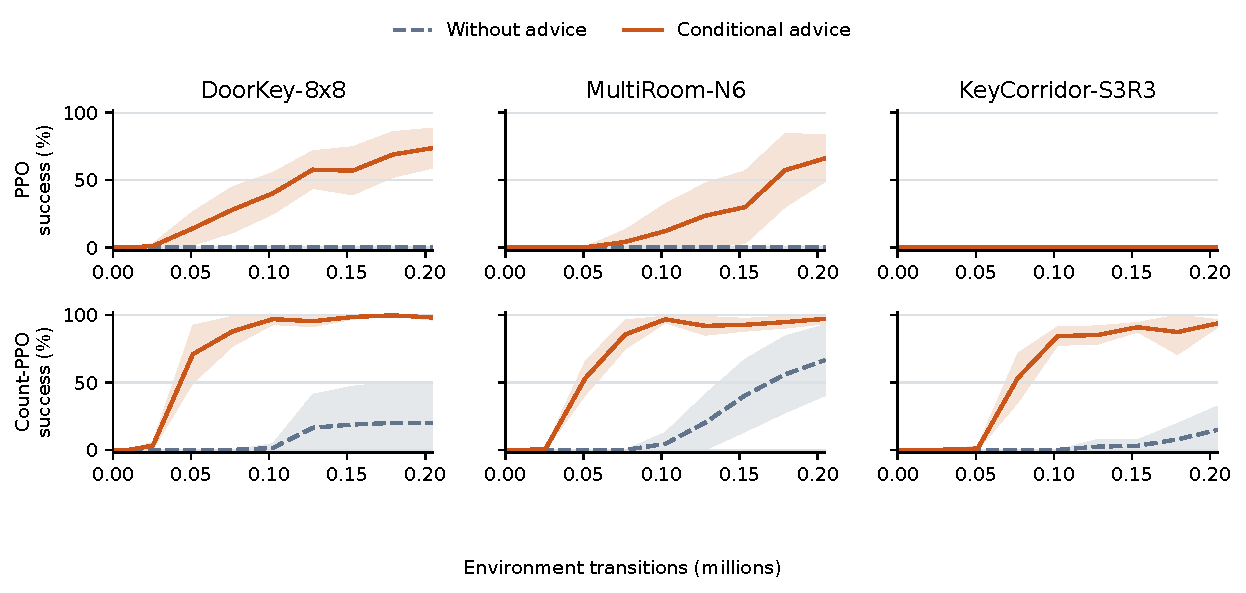
\includegraphics[width=1\linewidth,height=\textheight,keepaspectratio,alt={Fresh-cohort early greedy success on an ordinary linear axis, including measured initialization. Each panel uses ten training seeds per arm.}]{figures/source_fresh_early_greedy.pdf}
\caption{Fresh-cohort early greedy success on an ordinary linear axis,
including measured initialization. Each panel uses ten training seeds
per arm.}
\end{figure}

\begin{figure}
\centering
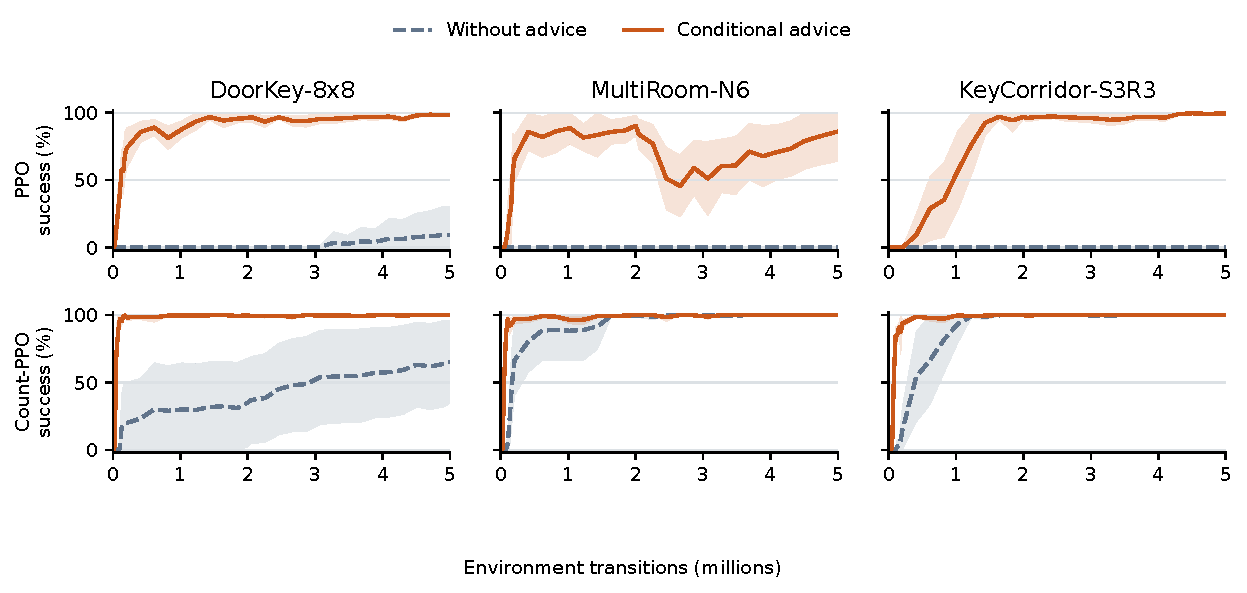
\includegraphics[width=1\linewidth,height=\textheight,keepaspectratio,alt={Fresh-cohort greedy success over the full training budget on a linear axis.}]{figures/source_fresh_linear_greedy.pdf}
\caption{Fresh-cohort greedy success over the full training budget on a
linear axis.}
\end{figure}

\begin{figure}
\centering
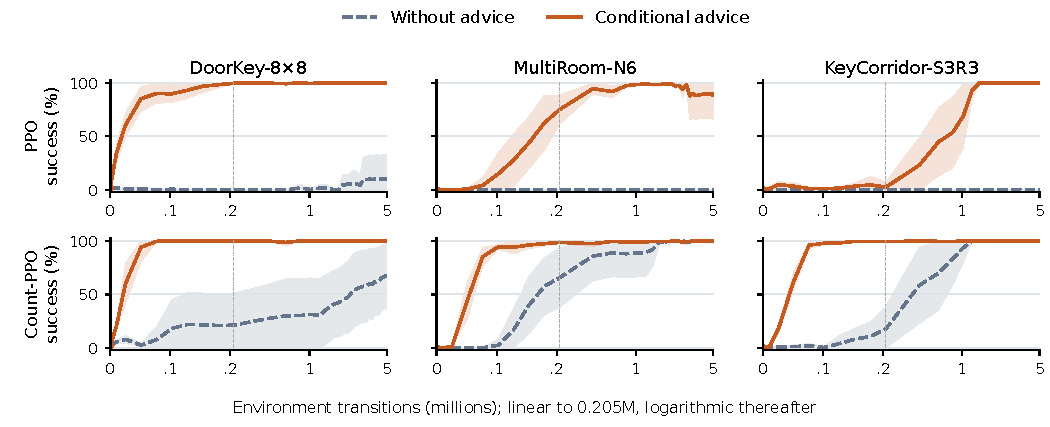
\includegraphics[width=1\linewidth,height=\textheight,keepaspectratio,alt={Sampled-action success on the same fresh cohort as the initialization diagnostics.}]{figures/source_fresh_sampled.pdf}
\caption{Sampled-action success on the same fresh cohort as the
initialization diagnostics.}
\end{figure}




The original confirmation-cohort sampled curves, including no advice, appear
in the main paper's combined four-method figure. The figures here retain
the fresh-cohort initialization measurements and are not spliced into that comparison.

\clearpage
\section{Generated-Controller Comparison}\label{generated-controller-comparison}

We adapt RLingua's teaching procedure to recurrent PPO and discrete actions,
rather than reproduce its original TD3 experiments. A's generated controller
reads full simulator state. B's controller reads local observations and its
memory; its writer additionally receives 36 fresh full-map example situations
paired with the student's view. These supply the same type of privileged
example information as our bank construction, not identical example layouts
or an otherwise identical generation process. B0 denotes the original
local-observation controller without that example message. Throughout the
main paper, B means the version with examples.

The controller acts with probability $0.25\,0.999999^n$ after $n$ transitions.
Its transitions supply replayed cross-entropy targets at weight 1.0. Student
policy/value losses exclude controller transitions and advantage traces stop
at them. Our bank labels student-visited states with a weight starting at
0.1, decreasing to 0.001 and removed at 75\% of training. Bank construction
and controller generation produce different artifacts; replay, intervention
and imitation schedules differ. KeyCorridor's bank executor also has an
explicit progress predicate. The comparison is between teaching procedures,
not an exact match isolating representation, abstention, or runtime information.

\subsection{Completed student comparisons}
The completed B suites are \texttt{dk\_rlex}, \texttt{mr\_rlex} and
\texttt{kc\_rlex}: ten paired seeds per student and task, 60 runs in total.
All reach 4,999,168 transitions. Each has 26 regular checkpoints, beginning
at 204,800; AUC is integrated on this common support. B and B0 training
arguments differ only in controller identity and experiment name. We verified
manifest identities, critical source/controller hashes, terminal summaries,
initial-policy hashes, seed pairing and teacher-free evaluation logs.
Paired-$t$ and Holm calculations were cross-checked against the frozen
producer functions. These completed values supersede the earlier partial
AUC read-outs.


\begin{table}[htbp]\centering\small

\caption{Mean greedy success AUC of completed students, ten paired training seeds per setting. No advice, our bank, full-state A, example-supplied B and original B0. Greedy AUC is the primary inferential metric.}

\label{tab:minigrid_teaching}

\begin{tabular}{@{}llrrrrr@{}}\toprule

Task & Student & No advice & Ours & A & B & B0\\\midrule

DoorKey-8x8 & PPO & 0.000 & 0.939 & 0.958 & 0.994 & 0.800\\

DoorKey-8x8 & Count-PPO & 0.569 & 0.992 & 1.000 & 1.000 & 0.977\\

MultiRoom-N6 & PPO & 0.000 & 0.767 & 0.815 & 0.002 & 0.000\\

MultiRoom-N6 & Count-PPO & 0.746 & 0.988 & 0.979 & 0.710 & 0.634\\

KeyCorridor-S3R3 & PPO & 0.000 & 0.733 & 0.935 & 0.594 & 0.587\\

KeyCorridor-S3R3 & Count-PPO & 0.956 & 0.994 & 0.995 & 0.921 & 0.666\\

\bottomrule\end{tabular}\end{table}

\begin{table}[htbp]\centering\small

\caption{Mean sampled success AUC of completed students, ten paired training seeds per setting. No advice, our bank, full-state A, example-supplied B and original B0. Sampled AUC is descriptive secondary evidence.}

\label{tab:sampled_controllers}

\begin{tabular}{@{}llrrrrr@{}}\toprule

Task & Student & No advice & Ours & A & B & B0\\\midrule

DoorKey-8x8 & PPO & 0.013 & 0.999 & 0.999 & 1.000 & 0.884\\

DoorKey-8x8 & Count-PPO & 0.604 & 1.000 & 1.000 & 1.000 & 0.994\\

MultiRoom-N6 & PPO & 0.000 & 0.976 & 0.914 & 0.002 & 0.000\\

MultiRoom-N6 & Count-PPO & 0.747 & 0.993 & 0.977 & 0.703 & 0.653\\

KeyCorridor-S3R3 & PPO & 0.000 & 0.819 & 0.997 & 0.683 & 0.698\\

KeyCorridor-S3R3 & Count-PPO & 0.962 & 0.999 & 1.000 & 0.964 & 0.693\\

\bottomrule\end{tabular}\end{table}



Each contrast family below has six comparisons. Intervals are unadjusted
paired-$t$ 95\% intervals; $p_H$ denotes the two-sided Holm-adjusted
$p$-value within that family. AUC differences are paired by training seed
and verified initial policy. The B families were specified in protocol
addendum 17 before its learning runs. The A/B0 families are addendum 16.


\begin{table}[htbp]\centering\small

\caption{Our bank minus B (with examples): completed greedy-AUC contrasts.}

\begin{tabular}{@{}llrrlr@{}}\toprule

Task & Student & $\Delta$AUC & Positive pairs & 95\% CI & $p_H$\\\midrule

DoorKey-8x8 & PPO & -0.055 & 1/10 & [-0.077, -0.032] & 0.00116\\

DoorKey-8x8 & Count-PPO & -0.008 & 0/10 & [-0.011, -0.004] & 0.00116\\

MultiRoom-N6 & PPO & +0.765 & 10/10 & [+0.702, +0.828] & 3.12e-09\\

MultiRoom-N6 & Count-PPO & +0.278 & 10/10 & [+0.189, +0.366] & 0.000222\\

KeyCorridor-S3R3 & PPO & +0.140 & 8/10 & [-0.025, +0.304] & 0.0877\\

KeyCorridor-S3R3 & Count-PPO & +0.073 & 10/10 & [+0.052, +0.095] & 0.000134\\

\bottomrule\end{tabular}\end{table}

\begin{table}[htbp]\centering\small

\caption{Our bank minus A (full state): completed greedy-AUC contrasts.}

\begin{tabular}{@{}llrrlr@{}}\toprule

Task & Student & $\Delta$AUC & Positive pairs & 95\% CI & $p_H$\\\midrule

DoorKey-8x8 & PPO & -0.020 & 1/10 & [-0.038, -0.001] & 0.127\\

DoorKey-8x8 & Count-PPO & -0.007 & 0/10 & [-0.011, -0.004] & 0.00412\\

MultiRoom-N6 & PPO & -0.048 & 3/10 & [-0.104, +0.007] & 0.162\\

MultiRoom-N6 & Count-PPO & +0.009 & 8/10 & [+0.004, +0.014] & 0.0157\\

KeyCorridor-S3R3 & PPO & -0.202 & 0/10 & [-0.298, -0.106] & 0.00524\\

KeyCorridor-S3R3 & Count-PPO & -0.000 & 6/10 & [-0.003, +0.003] & 0.942\\

\bottomrule\end{tabular}\end{table}

\begin{table}[htbp]\centering\small

\caption{B with examples minus original B0: completed greedy-AUC contrasts.}

\begin{tabular}{@{}llrrlr@{}}\toprule

Task & Student & $\Delta$AUC & Positive pairs & 95\% CI & $p_H$\\\midrule

DoorKey-8x8 & PPO & +0.194 & 10/10 & [+0.095, +0.293] & 0.00976\\

DoorKey-8x8 & Count-PPO & +0.023 & 10/10 & [+0.006, +0.040] & 0.0592\\

MultiRoom-N6 & PPO & +0.002 & 2/10 & [-0.002, +0.006] & 0.827\\

MultiRoom-N6 & Count-PPO & +0.077 & 5/10 & [-0.120, +0.274] & 0.827\\

KeyCorridor-S3R3 & PPO & +0.007 & 4/10 & [-0.106, +0.119] & 0.897\\

KeyCorridor-S3R3 & Count-PPO & +0.256 & 10/10 & [+0.106, +0.405] & 0.0192\\

\bottomrule\end{tabular}\end{table}

\begin{table}[htbp]\centering\small

\caption{Our bank minus original B0: completed greedy-AUC contrasts.}

\begin{tabular}{@{}llrrlr@{}}\toprule

Task & Student & $\Delta$AUC & Positive pairs & 95\% CI & $p_H$\\\midrule

DoorKey-8x8 & PPO & +0.139 & 10/10 & [+0.031, +0.247] & 0.0513\\

DoorKey-8x8 & Count-PPO & +0.015 & 7/10 & [-0.001, +0.032] & 0.128\\

MultiRoom-N6 & PPO & +0.767 & 10/10 & [+0.705, +0.829] & 2.69e-09\\

MultiRoom-N6 & Count-PPO & +0.354 & 10/10 & [+0.175, +0.534] & 0.00621\\

KeyCorridor-S3R3 & PPO & +0.146 & 8/10 & [-0.040, +0.332] & 0.128\\

KeyCorridor-S3R3 & Count-PPO & +0.329 & 10/10 & [+0.176, +0.481] & 0.00434\\

\bottomrule\end{tabular}\end{table}

\subsection{Interpretation and original-controller evidence}
Our advantage over B is supported on MultiRoom with both students and
KeyCorridor Count-PPO. B's DoorKey advantage is also significant; the
KeyCorridor PPO difference remains inconclusive. The Count-PPO differences
from A are below 0.01 in magnitude, without establishing equivalence.
A is significantly better for KeyCorridor PPO. These patterns support
conditional teaching as an effective design without a universal ranking.

In standalone controller evaluations on 100 layouts, B solves all DoorKey
layouts and none on MultiRoom or KeyCorridor. This establishes the quality
of these generated candidates, not an impossibility for local-observation
controllers. A local controller with memory can integrate information over
 time. No experiment isolates observation overlap as the cause of the
DoorKey result. We retain B0 to show what changes when example situations
are added to the writer's context.



\subsection{Executing actions from our own bank}
The separate same-bank execution variant retains imitation while sometimes
executing the rule target. Label-only teaching meets the declared 0.05 AUC
non-inferiority margin in five of six settings. For KeyCorridor PPO,
execution has a higher mean (0.896 versus 0.733), but the corrected contrast
is inconclusive ($p=0.126$). This variant uses student-policy probabilities
for mixed-policy actions in PPO, a known formulation limitation. It is
distinct from the controller adaptation above. Supplement Section 10 gives
both greedy and sampled curves and the execution schedule.


The main paper presents the sampled learning curves once. The tables here
report greedy and sampled AUC separately, including B0, without repeating
the controller figure.

\clearpage
\section{Progress Conditions and Advice
Quantity}\label{progress-conditions-and-advice-quantity}

\begin{longtable}[]{@{}
  >{\raggedright\arraybackslash}p{(\linewidth - 6\tabcolsep) * \real{0.2500}}
  >{\raggedleft\arraybackslash}p{(\linewidth - 6\tabcolsep) * \real{0.2500}}
  >{\raggedleft\arraybackslash}p{(\linewidth - 6\tabcolsep) * \real{0.2500}}
  >{\raggedleft\arraybackslash}p{(\linewidth - 6\tabcolsep) * \real{0.2500}}@{}}
\caption{Separate ten-seed advice-quantity control. Thinned-full minus
no-progress AUC is +0.720 {[}0.526, 0.914{]}, Holm-adjusted
\(p=.000038\). The aggregate retained-label ratio is 1.0048. Per-run
label counts are rounded means. This cohort differs from the original
and fresh source cohorts.}\tabularnewline
\toprule\noalign{}
\begin{minipage}[b]{\linewidth}\raggedright
KeyCorridor-S3R3, plain PPO
\end{minipage} & \begin{minipage}[b]{\linewidth}\raggedleft
AUC
\end{minipage} & \begin{minipage}[b]{\linewidth}\raggedleft
Final success (\%)
\end{minipage} & \begin{minipage}[b]{\linewidth}\raggedleft
Retained labels per run
\end{minipage} \\
\midrule\noalign{}
\endfirsthead
\toprule\noalign{}
\begin{minipage}[b]{\linewidth}\raggedright
KeyCorridor-S3R3, plain PPO
\end{minipage} & \begin{minipage}[b]{\linewidth}\raggedleft
AUC
\end{minipage} & \begin{minipage}[b]{\linewidth}\raggedleft
Final success (\%)
\end{minipage} & \begin{minipage}[b]{\linewidth}\raggedleft
Retained labels per run
\end{minipage} \\
\midrule\noalign{}
\endhead
\bottomrule\noalign{}
\endlastfoot
No advice & .000 & 0.0 & 0 \\
Full bank & .722 & 90.0 & 1,465,562 \\
No progress conditions & .019 & 8.6 & 1,073,271 \\
Randomly thinned full bank & .739 & 89.6 & 1,078,445 \\
\end{longtable}

Random thinning approximately matches aggregate retained advice
quantity, while retaining a large learning advantage for
progress-conditioned advice. It does not match the states visited, the
individual targets or gradient estimates. The full-bank reference mean
is slightly below the thinned-bank mean; this descriptive difference
does not establish that thinning improves learning.


\begin{figure}[htbp]\centering
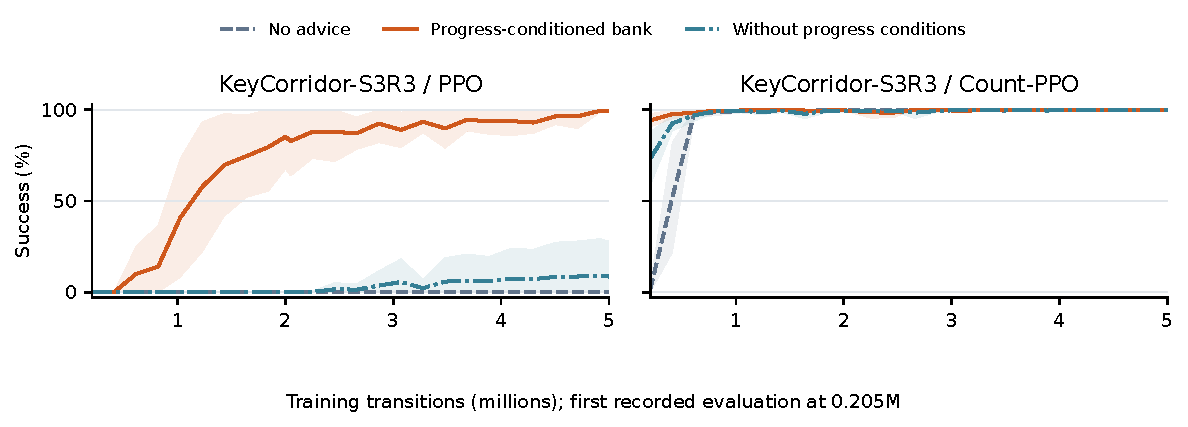
\includegraphics[width=\linewidth]{figures/progress_learning.pdf}
\caption{KeyCorridor progress-condition ablation, ten paired seeds and 5M transitions. Curves are mean teacher-free greedy success with pointwise unadjusted 95\% $t$-intervals across training seeds, clipped to the feasible range. Curve-band overlap is not a test of paired AUC differences.}
\end{figure}

\begin{figure}[htbp]\centering
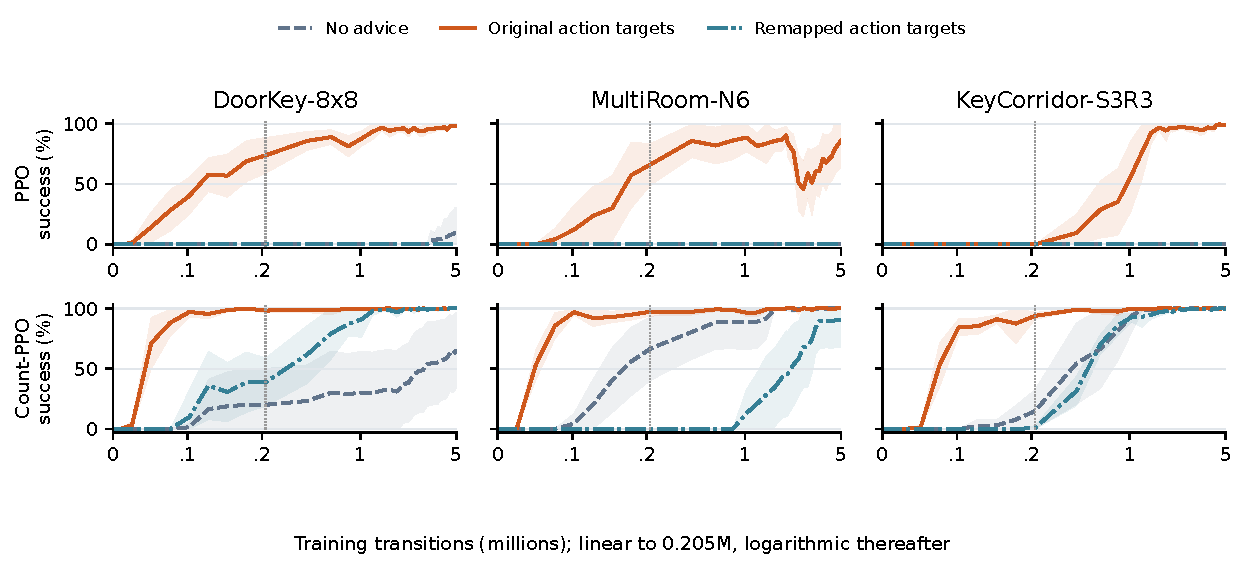
\includegraphics[width=\linewidth]{figures/content_learning.pdf}
\caption{Fresh action-content control, ten paired seeds per setting and 5M transitions. Measured initialization is included. The horizontal axis is linear through 204,800 transitions and logarithmic thereafter. Curves are mean teacher-free greedy success with pointwise unadjusted 95\% $t$-intervals across training seeds, clipped to the feasible range. Curve-band overlap is not a test of paired AUC differences.}
\end{figure}

\clearpage
\section{Online Advice at a Fixed Request
Budget}\label{online-advice-at-a-fixed-request-budget}

\begin{longtable}[]{@{}
  >{\raggedright\arraybackslash}p{(\linewidth - 10\tabcolsep) * \real{0.1667}}
  >{\raggedright\arraybackslash}p{(\linewidth - 10\tabcolsep) * \real{0.1667}}
  >{\raggedleft\arraybackslash}p{(\linewidth - 10\tabcolsep) * \real{0.1667}}
  >{\raggedleft\arraybackslash}p{(\linewidth - 10\tabcolsep) * \real{0.1667}}
  >{\raggedright\arraybackslash}p{(\linewidth - 10\tabcolsep) * \real{0.1667}}
  >{\raggedleft\arraybackslash}p{(\linewidth - 10\tabcolsep) * \real{0.1667}}@{}}
\caption{Online-advice comparison on ten fresh paired seeds per setting
at initial imitation weight 0.1. Request caps equal the selected bank's
construction-and-checking requests. The online model receives the same
full-map consultation prompt used for rule generation. The comparison
replaces the earlier unequal 15/12-pair study in the main
text.}\tabularnewline
\toprule\noalign{}
\begin{minipage}[b]{\linewidth}\raggedright
Task
\end{minipage} & \begin{minipage}[b]{\linewidth}\raggedright
Student
\end{minipage} & \begin{minipage}[b]{\linewidth}\raggedleft
Request cap
\end{minipage} & \begin{minipage}[b]{\linewidth}\raggedleft
Bank minus online AUC
\end{minipage} & \begin{minipage}[b]{\linewidth}\raggedright
95\% CI
\end{minipage} & \begin{minipage}[b]{\linewidth}\raggedleft
Holm-adjusted \(p\)
\end{minipage} \\
\midrule\noalign{}
\endfirsthead
\toprule\noalign{}
\begin{minipage}[b]{\linewidth}\raggedright
Task
\end{minipage} & \begin{minipage}[b]{\linewidth}\raggedright
Student
\end{minipage} & \begin{minipage}[b]{\linewidth}\raggedleft
Request cap
\end{minipage} & \begin{minipage}[b]{\linewidth}\raggedleft
Bank minus online AUC
\end{minipage} & \begin{minipage}[b]{\linewidth}\raggedright
95\% CI
\end{minipage} & \begin{minipage}[b]{\linewidth}\raggedleft
Holm-adjusted \(p\)
\end{minipage} \\
\midrule\noalign{}
\endhead
\bottomrule\noalign{}
\endlastfoot
DoorKey-8 & PPO & 62 & +.937 & {[}.921, .953{]} &
\(1.5\times10^{-15}\) \\
DoorKey-8 & Count-PPO & 62 & +.360 & {[}.038, .682{]} & .065 \\
MultiRoom-N6 & PPO & 36 & +.738 & {[}.655, .821{]} &
\(2.7\times10^{-8}\) \\
MultiRoom-N6 & Count-PPO & 67 & +.101 & {[}\ensuremath{-}.047, .250{]} & .156 \\
\end{longtable}

Online advice supplies mean label counts of 61.5 and 59.2 for DoorKey
PPO and Count-PPO, and 35.7 and 65.4 for the corresponding MultiRoom
students. Banks supply approximately 1.81M, 1.93M, 3.20M and 0.83M
labels per run, respectively. This is a request-budget comparison, not a
matched-supervision experiment. The reported selected-bank cost excludes
unused development candidates and student training compute.




\begin{figure}[tp]\centering
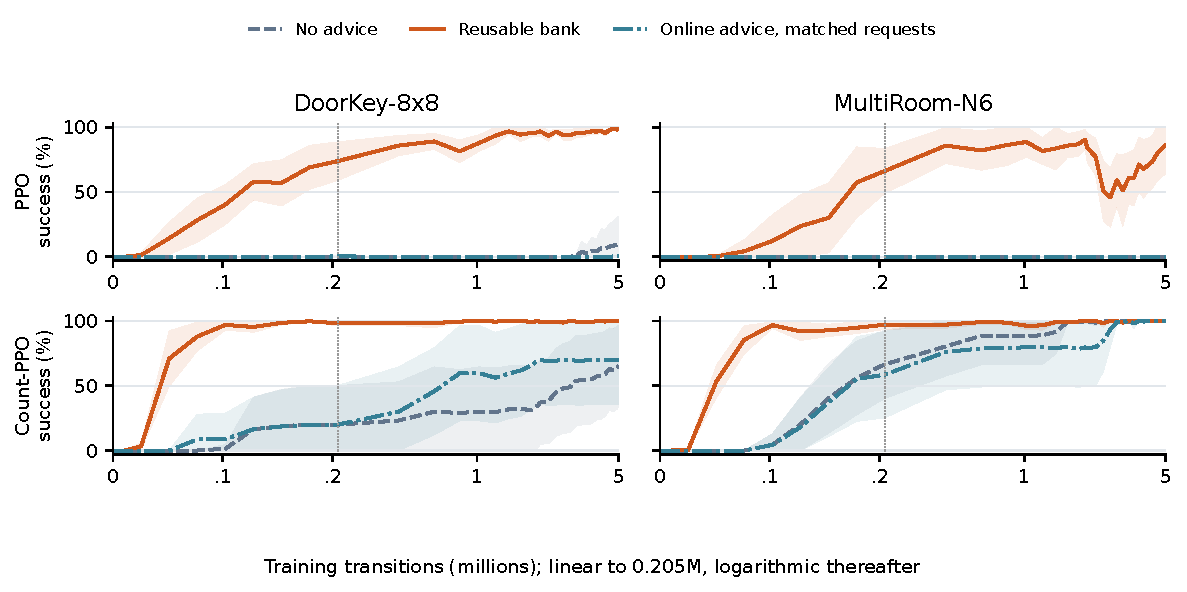
\includegraphics[width=\linewidth]{figures/online_learning.pdf}
\caption{Reusable bank versus online advice with a matched request cap. Ten fresh paired seeds per setting and 5M transitions. Initial and early checkpoints are measured; the axis is linear through 204,800 transitions and logarithmic thereafter. Curves are mean teacher-free greedy success with pointwise unadjusted 95\% $t$-intervals across training seeds, clipped to the feasible range. Curve-band overlap is not a test of paired AUC differences.}
\end{figure}

\clearpage
\section{Additional Crafter Results}\label{additional-crafter-results}

\begin{longtable}[]{@{}
  >{\raggedright\arraybackslash}p{(\linewidth - 4\tabcolsep) * \real{0.3333}}
  >{\raggedleft\arraybackslash}p{(\linewidth - 4\tabcolsep) * \real{0.3333}}
  >{\raggedright\arraybackslash}p{(\linewidth - 4\tabcolsep) * \real{0.3333}}@{}}
\caption{Additional symbolic-Crafter evidence. Fresh training uses ten
new training seeds and learning-average distinct achievements per
episode over 20 checkpoints. Fresh-world results evaluate the original
final policies on fifty additional worlds and measure endpoint
achievements. These are separate questions and metrics.}\tabularnewline
\toprule\noalign{}
\begin{minipage}[b]{\linewidth}\raggedright
Study and contrast
\end{minipage} & \begin{minipage}[b]{\linewidth}\raggedleft
Effect
\end{minipage} & \begin{minipage}[b]{\linewidth}\raggedright
95\% CI or reported scope
\end{minipage} \\
\midrule\noalign{}
\endfirsthead
\toprule\noalign{}
\begin{minipage}[b]{\linewidth}\raggedright
Study and contrast
\end{minipage} & \begin{minipage}[b]{\linewidth}\raggedleft
Effect
\end{minipage} & \begin{minipage}[b]{\linewidth}\raggedright
95\% CI or reported scope
\end{minipage} \\
\midrule\noalign{}
\endhead
\bottomrule\noalign{}
\endlastfoot
Fresh training: PPO, bank minus none & +.495 & {[}.293, .696{]}; Holm
\(p=.0011\) \\
Fresh training: Count-PPO, bank minus none & +.447 & {[}.296, .597{]};
Holm \(p=.00035\) \\
Fresh training: PPO, full minus no-progress bank & +.345 &
{[}.082,.608{]}; Holm \(p=.032\) \\
Fresh training: Count-PPO, full minus no-progress bank & +.190 &
{[}\ensuremath{-}.057,.436{]}; Holm \(p=.116\) \\
Fresh worlds: PPO, bank minus none & +.550 & {[}.158, .942{]}; Holm
\(p=.034\) \\
Fresh worlds: PPO, full minus no-progress bank & +.278 & {[}.060,
.496{]}; Holm \(p=.036\) \\
Fresh worlds: Count-PPO, bank minus none & +.200 & {[}\ensuremath{-}.135,.535{]};
Holm \(p=.21\) \\
\end{longtable}

Fresh-world PPO means are 6.800 with advice and 6.250 without advice;
Count-PPO means are 6.772 and 6.572. The fixed ten-world panel used
during learning is disjoint from the training worlds; the fifty
additional worlds provide a separate final-policy evaluation. In
development, direct bank execution with action preconditions achieved
3.55 achievements over 20 episodes, compared with 2.60 for random
actions. That diagnostic uses a different panel and is not a paired
comparison with the student results.



\clearpage
\section{Bank Regeneration and Aggregate Advice Rates}\label{sec:supp:bank_robustness}
Five additional DoorKey banks are evaluated with ten paired PPO seeds each.
Their mean AUC gains over no advice are .952, .821, .917, .727 and .723.
All five are retained; four complete the original generation attempt and
the fifth is recovered after a failed consultation. Recorded generation
and checking costs total approximately \$0.54 including the failed attempt
and recovery. This is an exploratory one-task, one-model study, not fifty
independent bank-generation trials.

The following rates are delivered labels divided by recorded executor
consultations in the fresh cohort, pooled across ten seeds per setting.
They measure aggregate non-abstention while advice is active, not coverage
of the entire state space, coverage over time, or the fraction of all
training transitions receiving labels.
\begin{center}\begin{tabular}{@{}lrr@{}}\toprule
Task & PPO & Count-PPO\\\midrule
DoorKey & 50.5\% & 54.2\%\\
MultiRoom & 86.6\% & 22.6\%\\
KeyCorridor & 41.7\% & 47.5\%\\\bottomrule
\end{tabular}\end{center}
MultiRoom uses separately selected banks for the two students. The rates
reflect the states each student visits, as well as the bank's conditions.

\clearpage
\section{Sensitivity to Bank Generation}
\label{app:bank_regeneration}

To examine dependence on a particular generated bank, we repeated
the fixed DoorKey writing and blind-checking procedure five times
using the same construction states. Each repetition constructs an
entire bank from 36 initial rule-generation calls and subsequent
checking requests. All five banks were retained for evaluation,
without selecting among them using student learning outcomes.
Bank 2 required a documented technical generation recovery before
training; it was retained as part of the fixed five-bank study.

Each bank taught PPO on ten fresh paired training seeds with a
5M-step training budget. Table~\ref{tab:bank_regeneration} reports
teacher-free sampled-action learning-curve area (AUC), compared
with the paired no-advice students. Sampled-action reporting is
a secondary choice made after inspecting the sampled and greedy
evaluations; greedy evaluation was the pre-specified primary mode.
AUC is normalized over the observed regular-checkpoint interval,
204{,}800--4{,}999{,}168 training steps.

\begin{table}[ht]
\centering\small
\caption{All five additional DoorKey banks. Mean paired sampled-AUC
gain over no advice and unadjusted 95\% paired-$t$ confidence interval
over ten training seeds for each bank.}
\label{tab:bank_regeneration}
\begin{tabular}{@{}lrr@{}}
\toprule
Bank & Mean $\Delta$AUC & 95\% CI\\
\midrule
0 & $+0.9506$ & $[+0.8685,+1.0326]$\\
1 & $+0.8546$ & $[+0.7474,+0.9617]$\\
2 & $+0.9234$ & $[+0.8001,+1.0467]$\\
3 & $+0.7747$ & $[+0.5763,+0.9730]$\\
4 & $+0.7854$ & $[+0.6752,+0.8957]$\\
\bottomrule
\end{tabular}
\end{table}

All five banks improved mean sampled AUC over no advice. This
exploratory result shows that the observed DoorKey benefit extends
beyond the originally selected bank under this fixed recipe and
construction corpus. It does not establish that arbitrary banks
work, or remove dependence on the earlier development of the
vocabulary, prompts and checking procedure. The five banks are
the generation repetitions; their 50 student runs are not 50
independent banks.

\clearpage
\section{Earlier Action-Advising and Execution Comparisons}
\label{sec:supp:earlier}

Before the conditional-bank experiments, we investigated selective
action advising. These studies have different training horizons,
cohorts and supervision procedures from the main bank study. We
report their within-study comparisons separately. This section also
reports action-execution variants and their evaluation protocols.

\subsection{Selective online action advising}
An earlier MultiRoom-N6 study compares no advice, entropy-based query
selection, probability correction at threshold .20, and uniform random
query times. The teacher is GPT-5-mini with full-map access; recommended
actions supply cross-entropy targets while the student chooses its own
actions. The study uses five paired seeds, recurrent PPO or Count-PPO,
9,999,360 transitions, an initial imitation coefficient of 1.0 and a maximum
of 480 consultations per guided run. These settings differ from the
current bank study and from its request-matched online comparison.



All plain-PPO evaluation curves remain at zero in this cohort. Count-PPO
mean AUC is .348 without advice, .989 with entropy, .992 with probability
correction, and .945 with random queries. Probability correction delivers
127.2 labels per run on average versus 428.8 for entropy, while each uses
480 consultations. This demonstrates the distinction between delivered
labels and teacher queries. These procedures retain an inherited
random-number coupling between advice scheduling and PPO updates, identified
in a later audit; effects should be attributed to the tested procedures
rather than solely to the semantic content of received labels.

\subsection{Learning curves and the meaning of mistake correction}
Probability correction delivers a usable teacher target $a^T$ only when
$\pi_\theta(a^T\mid x)<0.2$, following the entropy-based query mechanism.
Exact-disagreement correction, explored in other earlier studies, instead
requires disagreement between the sampled student action and the teacher
action. Neither criterion proves that the teacher is correct. Random
query times choose when to request advice; they do not replace environment
actions with random actions. The online advisor controls teaching
opportunities or delivery, while the conditional bank controls the
applicability of reusable recommendations.

For the earlier MultiRoom study, probability correction and entropy
selection both use 480 consultations per Count-PPO run, but deliver means
of 127.2 and 428.8 labels, respectively. Neither pre-specified advisor
contrast establishes superiority after its family adjustment, and similar
mean performance is not an equivalence result. The same procedures leave
plain PPO at zero observed success. Timing, delivered dose and the inherited
random-number coupling also differ; these are comparisons of whole
procedures, not an isolated test of mistake detection.






\subsection{DoorKey advisors, importance and historical controls}
This section shows the complete earlier DoorKey and MultiRoom
online-advisor curves. DoorKey includes exact disagreement in addition
to entropy, probability correction and random query times. All three
entropy/correction plain-PPO arms have zero greedy AUC and final success.
Random queries reach 19.2\% final mean success, from one successful seed;
the no-advice mean is 3.6\%. Count-PPO reaches 100\% final mean success
with entropy, probability correction, random queries and no advice, and
80\% with exact disagreement. These results prevent describing every
earlier method as unsuccessful, while retaining their difficulty in
teaching plain PPO reliably in this cohort.

In a separate earlier DoorKey oracle screen, ten seeds per condition use
historical RGB observations, recurrent PPO without count bonus and 10M
transitions. Every guided arm delivers 200 labels. Teacher-Q importance
uses $\max_a Q_T(s,a)-\min_a Q_T(s,a)$; top-two-gap importance uses one
minus the gap between the student's two largest action probabilities;
entropy importance uses uncertainty across its action distribution.
Exact disagreement and probability-threshold correction apply additional
mistake criteria. Early advice supplies the initial labels without those
selection rules. These are a free oracle's labels, not LLM-generated rules.

All eight conditions have zero final greedy success. Sampled final means
range from 1.0\% without advice to 14.2\% for exact disagreement.
Figure~\ref{fig:legacy_importance} shows both metrics. Only final recorded
evaluations are used here; training-episode rewards are not substituted
for teacher-free evaluation curves. Seeds 0--4 and 5--9 use two recorded
source revisions, retained as historical blocks. These results do not
establish a general ranking of importance criteria or a matched
comparison with our current symbolic-observation bank study.

\begin{figure}[htbp]\centering
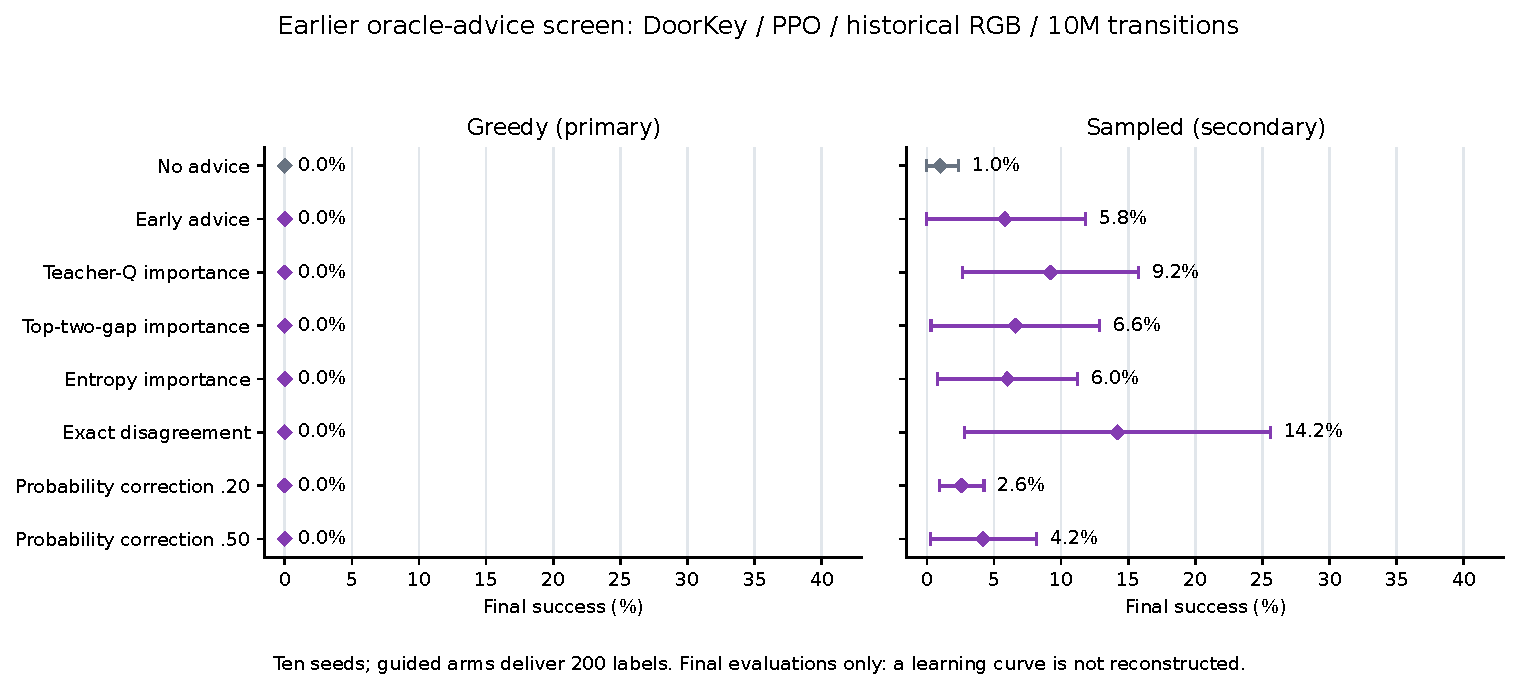
\includegraphics[width=\linewidth]{figures/legacy_importance_endpoints.pdf}
\caption{Historical oracle-advice screen: final teacher-free evaluation
of eight procedures, ten training seeds each, 10M transitions and 200
labels per guided run. Left: primary greedy success. Right: secondary
sampled success. Points are means with unadjusted 95\% $t$-intervals over
training seeds, clipped to the feasible range for display. The different
observation representation, teacher and code-revision blocks remain
explicit; this is not a current-bank baseline.}
\label{fig:legacy_importance}
\end{figure}

\subsection{Execution variants and evaluation comparability}
The current same-bank execution variant intermittently replaces the
student's action with the rule target while retaining the imitation loss.
The only non-identifier argument changes against the paired label-only
configuration are the execution start probability (0.75) and schedule
fraction (0.5). The probability is
$0.75\,0.01^{f/0.5}$ at training fraction $f$, until advice ends at $f=0.75$.
Its mixed behavior policy is scored using student-policy probabilities
in PPO. This known formulation limitation remains part of the reported
procedure. It is not the RLingua-style A/B implementation, which handles
controller transitions separately.

The same-bank comparison does not show that action execution is generally
unsuccessful. For example, it has mean greedy AUC 0.896 on KeyCorridor PPO,
versus 0.733 for label-only teaching; the paired contrast is inconclusive
after correction. Label-only teaching meets the declared 0.05 AUC
non-inferiority margin in five of the six settings. Figure~\ref{fig:execution_sampled}
adds sampled evaluation of the same trained students; primary paired
claims remain based on greedy AUC.

\begin{figure}[htbp]\centering
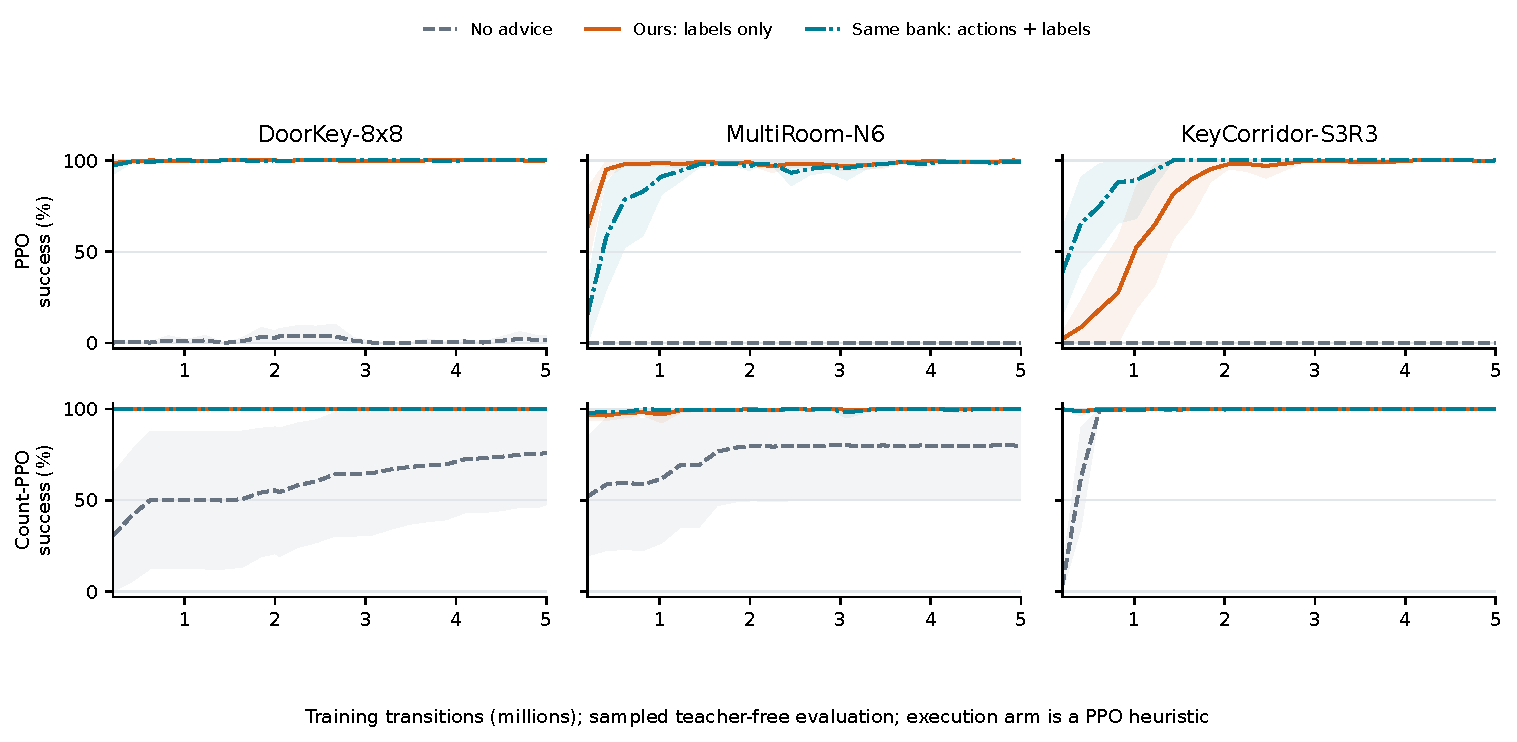
\includegraphics[width=\linewidth]{figures/bank_execution_sampled.pdf}
\caption{Secondary sampled-action evaluation of the same-bank teaching
comparison. Students and checkpoints match the greedy execution comparison below;
ten paired training seeds per task--student setting and 5M transitions.
Teaching is disabled during evaluation. Bands are pointwise 95\%
$t$-intervals clipped for display. The execution heuristic retains its
probability-accounting limitation.}
\label{fig:execution_sampled}
\end{figure}

Earlier override and teacher-prefix pilots are retained as historical
method-development records. Their channel comparisons used different
teacher-off measurements: dedicated greedy evaluation for distillation,
but recent stochastic training success after teacher removal for the
other channels. These quantities are not combined into a matched
performance plot. The present same-bank and A/B comparisons provide the
clearer action-execution evidence for the paper.


\begin{figure}[htbp]\centering
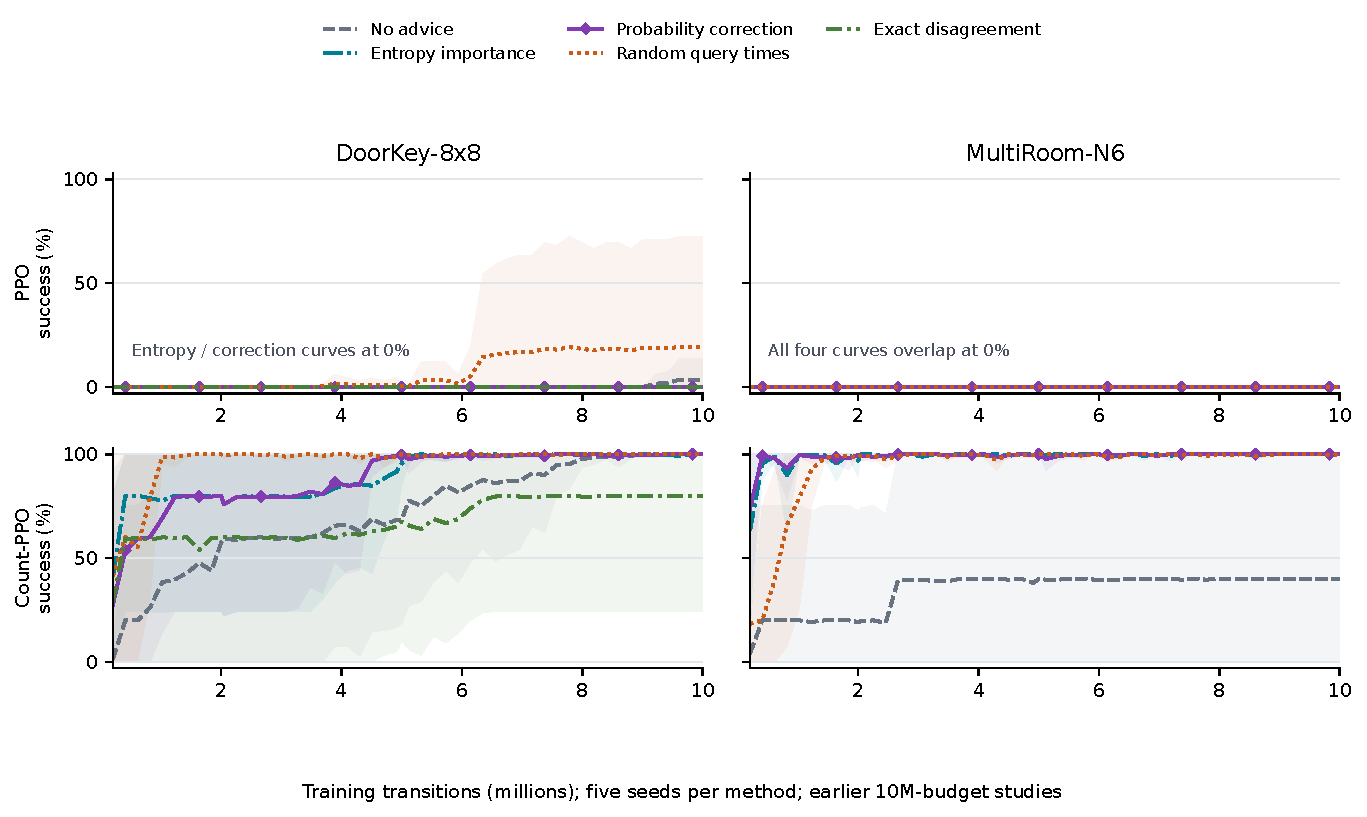
\includegraphics[width=\linewidth]{figures/earlier_online_advisors.pdf}
\caption{The earlier DoorKey and MultiRoom online-advisor studies, five
paired training seeds per method and 10M transitions. These are within-study
comparisons; cohorts and imitation settings differ from the current bank
study. Curves are mean greedy success with pointwise 95\% $t$-intervals.}
\end{figure}

\begin{figure}[htbp]\centering
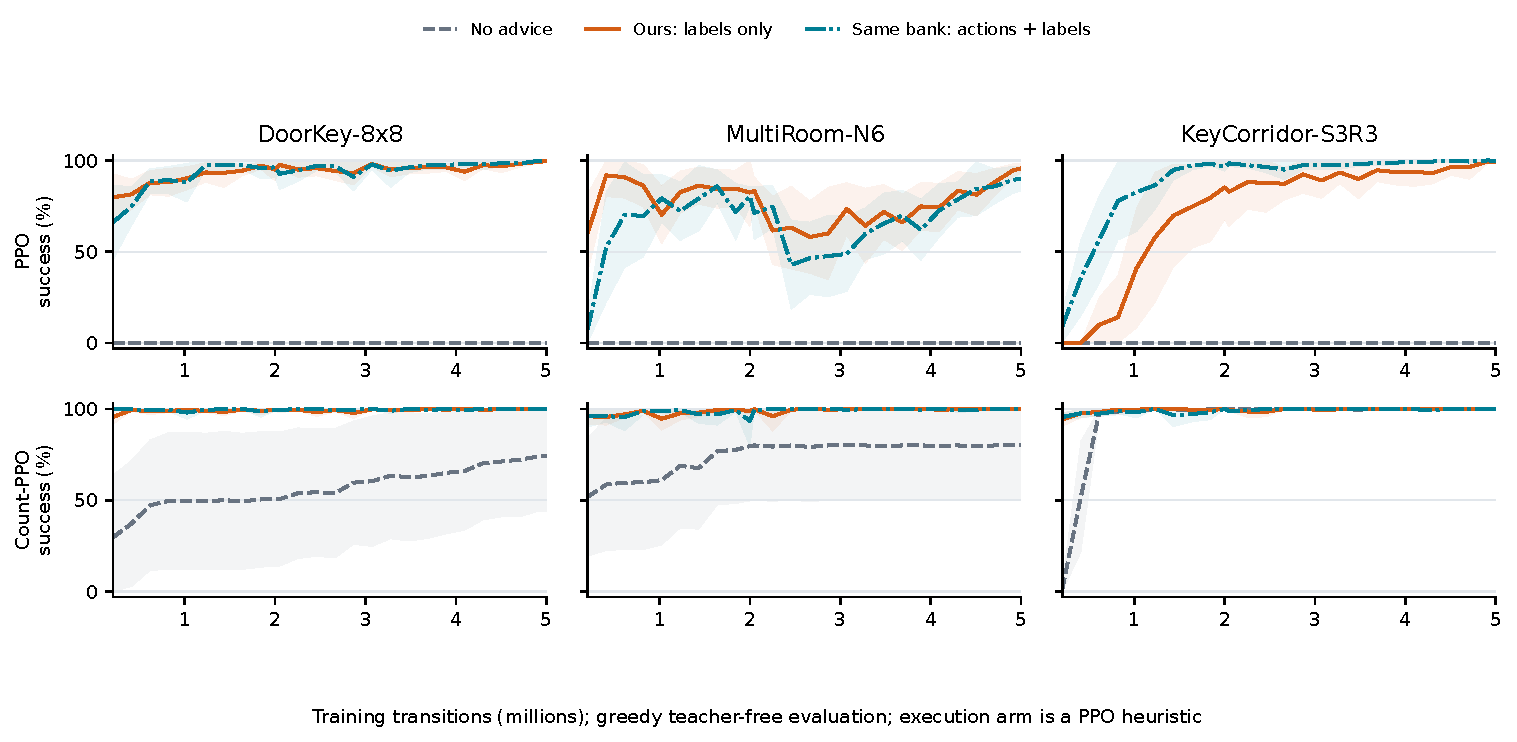
\includegraphics[width=\linewidth]{figures/bank_execution_greedy.pdf}
\caption{Same-bank greedy comparison of no advice, learning targets only,
and targets plus annealed action execution. Ten paired seeds per setting,
5M transitions, teacher-free evaluation. The execution variant retains
its known PPO probability-accounting limitation.}
\end{figure}

\subsection{Online advisors on all three tasks}
\label{sec:supp:online120}

We repeated the selective online-advising comparison on DoorKey-$8\times8$,
MultiRoom-N6 and KeyCorridor-S3R3 with at most 120 GPT-5-mini requests per
training run. All other settings follow the earlier study: a teacher with
full-map access, recurrent PPO or Count-PPO with local $7\times7$ symbolic
observations, 9,999,360 transitions, an imitation coefficient decaying from
1.0 to 0.01, and five paired training seeds per task. Entropy-based queries
request advice when the student's normalized policy entropy is high;
probability correction delivers the teacher's action as a target only when
the student assigns it probability below 0.2; random timing draws query
slots uniformly within the advice period. Delivered labels can be fewer
than requests. No-advice controls, the DoorKey and MultiRoom Count-PPO
random-timing runs and both KeyCorridor random-timing arms are completed
runs with identical settings and seeds. The remaining runs used a different
cluster: they share training seeds and settings with their controls but
not the initial network weights.

\begin{table}[htbp]\centering\small
\setlength{\tabcolsep}{4pt}
\caption{Online advisors with 120 requests per run: mean greedy AUC, with
mean final greedy success (\%) in parentheses. Five paired seeds, 10M
transitions.}
\label{tab:supp:online120}
\begin{tabular}{@{}llrrrr@{}}
\toprule
Task & Student & No advice & Entropy & Mistake corr. & Random \\
\midrule
DoorKey     & PPO       & .003 (3.6) & .000 (0) & .000 (0) & .000 (0) \\
            & Count-PPO & .719 (100) & .936 (100) & .864 (100) & .787 (100) \\
MultiRoom   & PPO       & .000 (0) & .000 (0) & .000 (0) & .000 (0) \\
            & Count-PPO & .348 (40) & .927 (100) & .948 (100) & .956 (99.6) \\
KeyCorridor & PPO       & .000 (0) & .000 (0) & .000 (0) & .000 (0) \\
            & Count-PPO & .936 (100) & .966 (100) & .980 (100) & .775 (80) \\
\bottomrule
\end{tabular}
\end{table}

Paired Count-PPO AUC gains over no advice (entropy, mistake correction,
random) are $+.216$, $+.145$ and $+.068$ on DoorKey; $+.579$, $+.600$ and
$+.608$ on MultiRoom; and $+.030$, $+.045$ and $-.161$ on KeyCorridor. No
gain is significant after Holm correction over the three advisors (smallest
adjusted $p=.138$). The earlier 480-request cohorts agree: with entropy
queries or mistake correction, plain PPO has 0\% final success on DoorKey
and MultiRoom, and random timing reaches 19.2\% on DoorKey from one seed.
The 8,395 requests cost \$32.25. Failed requests are 0.1\% on DoorKey and
about 8\% on MultiRoom and KeyCorridor, mostly replies cut off at the
output limit; a failed request delivers no label.

\begin{figure}[htbp]\centering
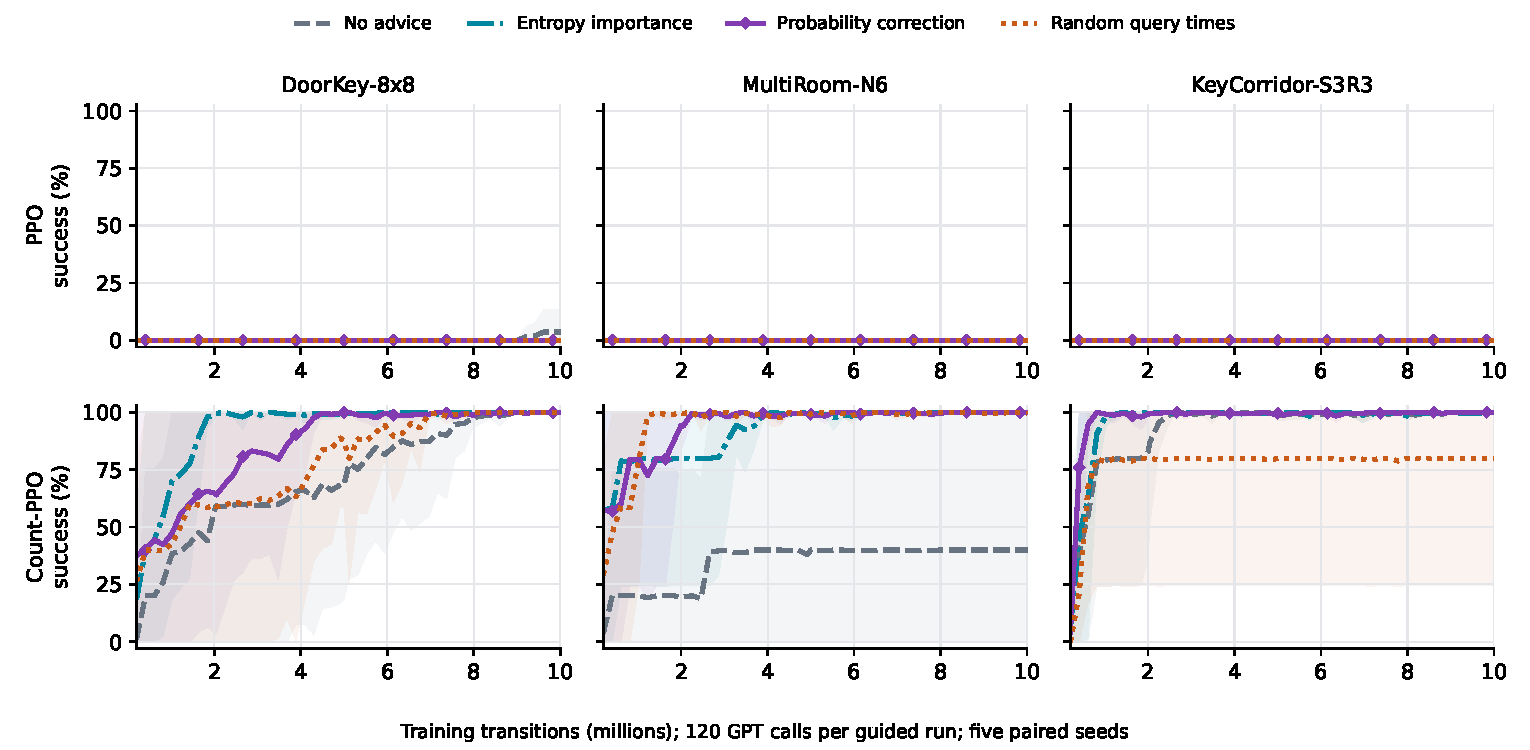
\includegraphics[width=\linewidth]{figures/online_advisors_120calls.pdf}
\caption{Online GPT-5-mini advisors with 120 requests per run on the three
source tasks. Teacher-free greedy success; lines are means over five
paired seeds and bands pointwise 95\% $t$-intervals clipped to
$[0,100]\%$. Plain PPO remains at 0\% with every advisor.}
\label{fig:supp:online120}
\end{figure}


\clearpage
\section{Fixed-Policy Baselines and Recorded Timing}
\label{app:baselines_timing}
\subsection{Random actions and direct bank execution}
The source-task evaluations run the fixed bank as a policy, executing its
target when available and choosing uniformly from the six non-\texttt{done}
actions otherwise. A separate baseline uses those random actions at every
step. Each source evaluation uses 200 episodes with seeds starting at
35,000,000. These are episode-level diagnostics of a fixed artifact, not
ten independent training runs. The student curves in the main paper are
teacher-free evaluations from separate panels; the separate fixed-policy scores
are not paired significance comparisons or learning curves.
\begin{center}\small
\begin{tabular}{@{}lrrr@{}}\toprule
Task & Random actions & PPO bank alone & Count-PPO bank alone\\\midrule
DoorKey-8 & 2.5\% & 66.0\% & 66.0\%\\
MultiRoom-N6 & 0.0\% & 5.5\% & 0.0\%\\
KeyCorridor-S3R3 & 0.5\% & 22.5\% & 22.5\%\\\bottomrule
\end{tabular}\end{center}
On larger maps, recorded 100-episode random-action success is 3\% on
DoorKey-16 and zero on MultiRoom-N10 and KeyCorridor-S6R3. Random-action
evaluations for S4R3 and S5R3 are not included in these records. Both
MultiRoom-N10 banks have zero standalone successes on their 100-episode
panel. The separate Crafter development diagnostic reports 2.60
achievements for random actions and 3.55 for the action-filtered bank on
20 worlds; this is not the students' held-out evaluation panel.

\subsection{Recorded construction and training times}
The regeneration journals provide an observed request window: earliest
request start to latest request completion across consultation and blind
checking. The per-request durations are also summed; concurrent calls
make this sum longer than the elapsed window. The four uninterrupted banks
have request windows of 1.17--1.59 minutes. These measurements exclude
queueing, pre-request setup, development and manual recovery delays.
Bank 2's original generation fails and is subsequently recovered; it is
retained in the learning results but has no single uninterrupted window
in this table. Each bank trains ten new PPO students to 4,999,168
transitions on CPU. Their median recorded elapsed times are listed below.

\begin{center}\small
\begin{tabular}{@{}lrrr@{}}\toprule
Bank & Request window (min) & Summed requests (min) & Median training (h)\\\midrule
0 & 1.19 & 6.56 & 4.16 \\
1 & 1.17 & 6.38 & 4.23 \\
2 & interrupted & interrupted & 4.13 \\
3 & 1.23 & 6.51 & 4.28 \\
4 & 1.59 & 7.60 & 4.17 \\
\bottomrule\end{tabular}\end{center}
These are descriptive timings from the recorded execution environment,
not a hardware-matched end-to-end speedup benchmark. They quantify one
construction stage and subsequent student training separately. A bank can
be reused across students; executor and auxiliary-loss computation still
occur during training. The time comparison does not include all development
or failed-bank exploration costs.


\bibliography{references.bib}

\end{document}
